\documentclass[mathserif, aspectratio=169, xcolor=table]{beamer}

\usepackage{psfrag,graphicx}
\usepackage{amsmath}
\usepackage[absolute,overlay]{textpos}

\usepackage{braket}
\graphicspath{{figs/}}

\usetheme{Boadilla}
\makeatother
\setbeamertemplate{footline}[frame number]

\usepackage{graphicx}
\usepackage{caption}
\usepackage{subcaption}
\captionsetup{compatibility=false}
\usepackage{amsmath} 
\usepackage{amssymb} 
\usepackage{amsthm}  
\usepackage{bm}
\usepackage{lipsum}
\usepackage[linesnumbered, ruled]{algorithm2e}
\usepackage{color}
\usepackage[normalem]{ulem}
\newtheorem{assumption}{Assumptions}
\newtheorem{prop}{Proposition}
\newtheorem{defn}{Definition}
\newtheorem{thm}{Theorem}
\newtheorem{lem}{Lemma}
\newtheorem{cor}{Corollary}
\newtheorem{sol}{Decentralized Solution}
\newtheorem{thresh}{$\epsilon$-thresholding}
\definecolor{light-gray}{gray}{0.8}
\usepackage{textcomp}

\newcommand{\backupbegin}{
   \newcounter{finalframe}
   \setcounter{finalframe}{\value{framenumber}}
}
\newcommand{\backupend}{
   \setcounter{framenumber}{\value{finalframe}}
}
\newcommand{\norm}[1]{\left\lVert #1 \right\rVert}

\makeatletter
\setbeamertemplate{navigation symbols}{}

\title[Lecture 22] % (optional, use only with long paper titles)
{Data, Environment and Society: \\{Lecture 22: Measuring Classifier Performance}}



\author[ER131: Data, Environment and Society] 
{Instructor: Duncan Callaway\\
GSI: Salma Elmallah} 

%\logo{
%\includegraphics[width=1.5cm,height=1.5cm,keepaspectratio]{uvic_logo_h.jpg}
%}
\vspace{-20mm}
\institute[UC Berkeley] % (optional, but mostly needed)
 {\small{ \bf November 14, 2019}}

\date[November 14, 2019]

\begin{document}

\frame{
	\titlepage
}

\begin{frame}{Announcements}
	\begin{itemize}
		\item Today: 
		\begin{itemize}
			\item Quick discussion of classifier performance, with notebook
			\item Exam review
		\end{itemize}
		\item HW10 posts today, due Tuesday before Thansksgiving (11/26)
		\item Lab next week: Cancelled, prep for exam!  Salma will hold special office hours.
		\item Tuesday next week: Exam
		\begin{itemize}
			\item Covers up to Lecture \sout{19} 21
			\item Covers up to HW9
		\end{itemize}
	\end{itemize}
\end{frame}


\begin{frame}{Objectives for today}
	\begin{itemize}
		\item Methods for measuring performance of classifiers
		\item Reminders on parameter, hyperparameter tuning
	\end{itemize}
	
\end{frame}

\begin{frame}{Reminder: classification error rate}

\pause
	The typical error, $\text{RSS} = \sum_{i=1}^N (y_i-\hat{y}_i)^2$ won't work.  \\~\\

	Alternatives?  Let's start by defining 
	\begin{align*}
	p_{mk} = \text{ fraction of observations belonging to class $k$ in region $m$.}
	\end{align*}
	Then a simple measure is:

	\begin{center}
	\textit{Classification error rate} = how many training observations don't fall into the assigned class.   \\~\\
	\end{center}

	 Within-region this is simply:

	\begin{align*}
	E_m = 1- \max_k (\hat{p}_{mk})
	\end{align*}
\end{frame}

\begin{frame}{The confusion matrix}
	\begin{itemize}
		\item A ``confusion matrix'' $C$ is such that $C_{i,j}$ is equal to the number of observations known to be in group $i$ but predicted to be in group $j$.
		\item Numbers on the diagonal of the matrix are correct predictions
		\item Rows sum to the number of actual observations in a category
		\item Columns sum to the number of predicted observations in a category
	\end{itemize}

% Please add the following required packages to your document preamble:
% \usepackage[table,xcdraw]{xcolor}
% If you use beamer only pass "xcolor=table" option, i.e. \documentclass[xcolor=table]{beamer}
\begin{table}[]
\begin{tabular}{l|l|l|}
\cline{2-3}
                                               & \cellcolor[HTML]{EFEFEF} Predict: True & \cellcolor[HTML]{EFEFEF} Predict: False \\ \hline
\multicolumn{1}{|l|}{\cellcolor[HTML]{EFEFEF}Actual: True} &      True pos (TP)                    &                False neg (FN)          \\ \hline
\multicolumn{1}{|l|}{\cellcolor[HTML]{EFEFEF}Actual: False} &           False pos (FP)              &               True neg (TN)           \\ \hline
\end{tabular}
\end{table}

\end{frame}

\begin{frame}{Precision and recall}
\begin{table}[]
\begin{tabular}{l|l|l|}
\cline{2-3}
                                               & \cellcolor[HTML]{EFEFEF} Predict: True & \cellcolor[HTML]{EFEFEF} Predict: False \\ \hline
\multicolumn{1}{|l|}{\cellcolor[HTML]{EFEFEF}Actual: True} &      True pos (TP)                    &                False neg (FN)          \\ \hline
\multicolumn{1}{|l|}{\cellcolor[HTML]{EFEFEF}Actual: False} &           False pos (FP)              &               True neg (TN)           \\ \hline
\end{tabular}
\end{table}


\begin{itemize}
	\item \textbf{Precision:} Correct number of positives divided by total number of positive predictions. 
	This is a ``true positive rate'': How many things classified as positive are actually positive?

	\begin{align*}
		 = \frac{TP}{TP+FP}
	\end{align*}


	\item \textbf{Recall:} Correctly number of positives divided by total number of true positives. \\
	This is $(1 -$ false positive rate$)$: How many positive outcomes are classified as positive?

	\begin{align*}
		 = \frac{TP}{TP+FN}
	\end{align*}

\end{itemize}

\end{frame}



\begin{frame}{Reminder / clarification for cross validation:  Models have two different classes of parameters}
	\begin{enumerate}
		\item Parameters that enter as decision variables for minimizing loss function:
		\begin{align*}
			\text{Shrinkage: } & \beta^*  &=& \arg \min_\beta \sum_{i=1}^N \left(Y_i - X_i \beta \right)^2+\lambda \cdot R(\beta)\\
			\text{CART: } & \{j^*,s^*\}  &=& \arg \min_{j\in J, s\in X_j} \sum_{i:x_i\in R_1(j,s)} (y_i-\hat{y}_{R_1})^2 + \sum_{i:x_i\in R_2(j,s)} (y_i-\hat{y}_{R_2})^2
		\end{align*}
		\item ``Hyperparameters'': parameters that constrain how you solve the loss function.  These generally prevent overfit.
		\begin{itemize} \pause
			\item $\lambda$ in shrinkage methods
			\item How deep to grow a classification tree?
			\item $\sum_{i=1}^n \epsilon_i$ in SVM
		\end{itemize}
	\end{enumerate}
	
\end{frame}

\begin{frame}{Ways to minimize the loss function}
\pause
	\begin{itemize}
		\item Closed form solution -- e.g. normal equations
		\item Gradient search
	\end{itemize}


	In both cases, we're relying on the condition that the gradient of the loss function approaches zero as we approach the optimal solution 
\end{frame}


\begin{frame}{Ways to choose hyperparameters}
\pause
	\begin{columns}
		\column{0.5\textwidth}
			\begin{itemize}
				\item \textbf{Grid search}: This is what we've done with shrinkage methods, when there is just one parameter to tune ($\lambda$)
				\item \textbf{Randomized parameter search}: This is what you're doing in HW10.  Works well when you have lots of hyperparameters to tune.
			\end{itemize}
		\column{0.5\textwidth}
			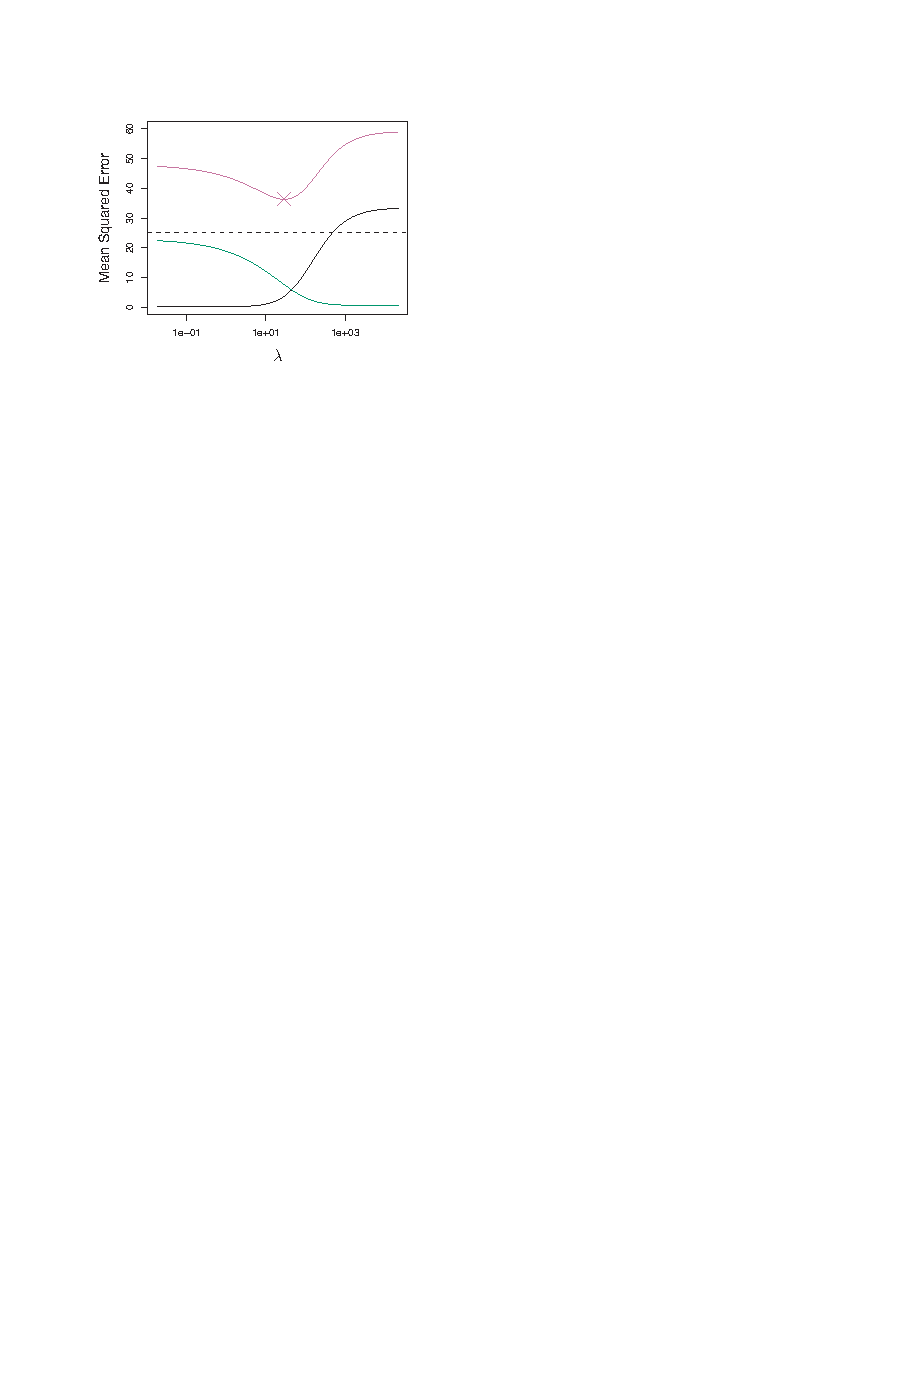
\includegraphics[width=0.9\textwidth]{bias-variance-ridge}
	\end{columns}
	In both cases, all we're doing is 
	\begin{itemize}
		\item Creating a list of candidate hyperparameters (or sets of hyperparameters)
		\item Training the model (with the training data) for each hyperparameter in the list
		\item Choosing the hyperparameter with the best cross-validated error.
	\end{itemize}
\end{frame}



\end{frame}


\begin{frame}{}
    
Let's look at this in a notebook (L22.ipynb)

\end{frame}
\end{document}
